% !TeX root = ExtendedAbstract.tex

\section{Background}

\subsection{Persistence Homology}

Persistence homology is a tool developed around 1992 for the purpose of data science. Data scientists had the need to compute the homology of a shape given a finite collection of data points $X$, which raises the question of finding a shape which adequately describes the data. A primitive algorithm consists of picking a positive number $r$ and replacing each data point by a sphere of radius $r$. The resulting open set, denoted $X^{(r)}$, may be understood as an approximation of the real shape underlying the data $X$, and there are efficient algorithms to compute its homology.

\begin{figure}
\centering
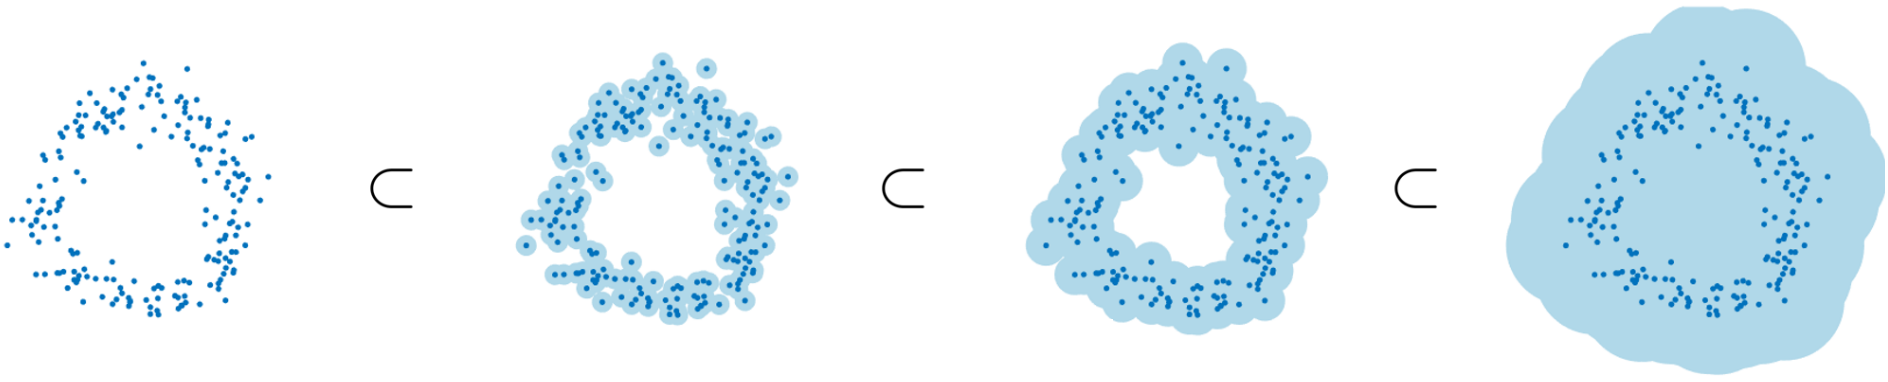
\includegraphics[width=\linewidth]{data}
\caption{Illustration of the sets $X^{(r)}$, with increasing $r$. Note that the middle radii are the ones which better represent the topology of the data. Figure taken from \cite{historypersistence}.}
\end{figure}

This raises the question of which radius $r$ to pick, which requires careful analysis of the data: too small $r$ and the datapoints will be disconnected, too large $r$ and the dataset degenerates into a large ball. However, persistence homology offers an alternative: consider all positive radii at once.

For $k \in \Z$ and $r > 0$, define $H_k^r(X) = H_k(X^{(r)})$, and for $r \leq 0$ set $H_k^r(X) = 0$. These spaces allow us to visualize how the shape of $X^{(r)}$ changes as $r$ increases. Moreover, for $r < s$ the inclusion $X^{(r)} \subseteq X^{(s)}$ induces a natural map $H_k^r(X) \to X_k^s(X)$. This data forms an object which is called a \emph{persistence module}. In the sequence we will be working exclusively with vector spaces, so assume that the homology is taken with coefficients over a field $\FF$.

\begin{definition}
A persistence module is a family of vector spaces $\{V_t\}_{t \in \R}$ (over a field $\FF$), together with maps $\pi_{st} \colon V_s \to V_t$ for $s \leq t$, such that
\begin{align}
\pi_{tt} &= \id,\\
\pi_{tr} \circ \pi_{st} &= \pi_{sr}, \quad s \leq t \leq r.
\end{align}

Moreover, a persistence module $(\{V_t\}_{t \in \R}, \{\pi_{st}\}_{s\leq t})$ is said to be of \emph{finite type} if the following three conditions are satisfied:
\begin{enumerate}
\item For all but finitely many $t$ there exists a neighborhood $U$ of $t$ such that $\pi_{st}$ is an isomorphism for $s, t \in U$,
\item For all $t \in \R$ there exists $\varepsilon$ such that $\pi_{(t-\delta), t}$ is an isomorphism for all $0 \leq \delta < \varepsilon$,
\item\label{pm3} For all $t \in \R$ close enough to $-\infty$, $V_t = 0$.
\end{enumerate}
\end{definition}

In practice, all the constructions for persistence modules that will be discussed in this thesis originate persistence modules of finite type. This is useful because of an important representation theorem for this class of persistence modules.

\begin{definition}
A \emph{barcode} is a finite multiset\footnote{A multiset is a set whose elements are counted with multiplicity.} of intervals of type $\linterval a b$, with $-\infty < a < b \leq +\infty$. We work under the convention that $\linterval a \infty = \ointerval a \infty$.
\end{definition}

\begin{definition}
Let $B = \{I_1, \dots, I_n\}$ be a barcode. Define the persistence module $\FF(B) = (\{V_t\}_{t \in \R}, \{\pi_{st}\}_{s \leq t})$ as follows
\begin{itemize}
\item Define $V_t = \braket{\,i \mid t \in I_i\,}$, where the brackets denote the free vector space over $\FF$,
\item For $s \leq t$, define $\pi_{st} \colon V_s \to V_t$ by defining it on the basis elements of $V_s$. For every $i$ such that $s \in I_i$,
\begin{itemize}
\item If $t \in I_i$, set $\pi_{st}(i) = i$,
\item Otherwise, set $\pi_{st}(i) = 0$.
\end{itemize}
\end{itemize}

It is straight-forward to prove that $\FF(B)$ is a persistence module of finite type.
\end{definition}

\begin{theorem}[Normal Form Theorem]
Every persistence module of finite type is isomorphic to $\FF(B)$ for exactly one barcode $B$.
\end{theorem}

The normal form theorem is the persistence analogous to the classical theorem in linear algebra that says that every vector space of finite dimension is isomorphic to $\R^n$ for some unique $n$. By property \ref{pm3} of finite type persistence modules, every persistence module `starts out' as the zero vector space, and at some instant in time it `grows a new basis element'. This marks the start of a bar in its barcode. Similarly, whenever the vector space $V_t$ loses a dimension, that is marked by the end of a bar. In this sense, the barcode of a persistence module is an indicator of when dimensions are appearing and disappearing; when applied to the homology of a topological space, \emph{the bars mark the appearance and disappearance of holes in the space as the parameter varies}.

\medskip

Another example, this one of a more geometrical nature, consists of considering a topological space equipped with a sufficient regular fibration, such as one induced by a Morse function. More concretely, let $X$ be a compact manifold and $f \colon X \to \R$ a Morse function on $X$. Define $X_t$, for $t \in \R$, as
\begin{equation}
X^t = \{\, x \in X \mid f(x) < t \,\}.
\end{equation}

Then, for $k \in \Z$ we may define a persistence module by
\begin{equation}
V_t = H_k(X_t),
\end{equation}
with the maps $\pi_{st} \colon V_s \to V_t$ being induced by the inclusion $X_s \hookrightarrow X_t$.

Elementary properties of Morse functions will show that the resulting persistence module is of finite type, and therefore has an associated barcode; this barcode is referred to as \emph{the barcode of $f$} (of dimension $k$).

As a concrete example, let $X$ be the torus, embedded vertically in $\R^3$ as in figure \ref{fig:torus1}. We will calculate the barcode (in dimension $1$) of the height function, whose critical values are $z_1 < z_2 < z_3 < z_4$.
\begin{figure}
\centering
\begin{tikzpicture}
\draw[->] (-2,-3) -- (-2,3.5) node[right] {$z$};

\draw (0,0) ellipse (1.5 and 2.7);
  \begin{scope}
    \clip (1.4,0) ellipse (1.8 and 3);
    \draw[name path global=p1] (-1,0) ellipse (1.2 and 2);
  \end{scope}
  \begin{scope}
    \clip (-1,0) ellipse (1.2 and 2);
    \draw[name path global=p2] (1,0) ellipse (1.2 and 2);
  \end{scope}
  
  
\draw[dashed] (0, 2.7) -- (-1.9, 2.7);
\draw (-1.9,2.7) -- (-2.1,2.7) node[left] {$z_4$};

\draw[dashed] (0, -2.7) -- (-1.9, -2.7);
\draw (-1.9,-2.7) -- (-2.1,-2.7) node[left] {$z_1$};

\node (origin) at (0,0) {};
\node (tr) at (-1.9,0) {};
\node (tl) at (-2.1,0) {};


\path [name intersections={of=p1 and p2}];


\draw[dashed] (origin |- intersection-1) -- (tr |- intersection-1);
\draw (tr |- intersection-1) -- (tl |- intersection-1) node[left] {$z_3$};

\draw[dashed] (origin |- intersection-2) -- (tr |- intersection-2);
\draw (tr |- intersection-2) -- (tl |- intersection-2) node[left] {$z_2$};


\end{tikzpicture}
\caption{An embedding of a torus in $\R^3$}\label{fig:torus1}
\end{figure}

Then, the filtration $X_t$ has the following behavior:
\begin{itemize}
\item For $t \leq z_1$, $X_t = \emptyset$, whose first homology is null;
\item For $z_1 < t \leq z_2$, $X_t$ is a disk, whose first homology is null;
\item For $z_2 < t \leq z_3$, $X_t$ is homeomorphic to a cylinder, and therefore its first homology is $\FF$,
\item At $t = z_3$, a handle is closed, and therefor for $z_3 < t \leq z_4$, $X_t$ has first homology equal to $\FF^2$,
\item Finally, for $t > z_4$ we obtain the full torus, whose first homology is $\FF^2$.
\end{itemize}

The induced maps $\pi_{st}$ can also be computed without much difficulty: they are the inclusions $\FF^n \hookrightarrow \FF^m$.

Now, the value of barcodes makes itself clear, as it allows for a much shorter description of the persistence module above described. The barcode associated to the height function in dimension $1$ is as follows:
\begin{figure}[H]
\centering
\begin{tikzpicture}[xscale=3]
\draw[->,thick] (-0.300,0.000)--(3.300,0.000);
\draw[] (0.000,-0.200)--(0.000,0.200) node[above] {$z_1$};
\draw[] (1.000,-0.200)--(1.000,0.200) node[above] {$z_2$};
\draw[] (2.000,-0.200)--(2.000,0.200) node[above] {$z_3$};
\draw[] (3.000,-0.200)--(3.000,0.200) node[above] {$z_4$};
\draw[(-,thick] (1.000,-0.500)--(3.255,-0.500) node[right] {};
\draw[(-,thick] (2.000,-0.800)--(3.255,-0.800) node[right] {};
\end{tikzpicture}
\caption{Visual representation of the barcode associated to the first homology of the torus in \ref{fig:torus1}.}\label{fig:bctorus}
\end{figure}

\subsection{Filtered Floer Homology}
\label{sec:ph}

Floer homology was developed by Andreas Floer in 1988 in order to attack the so-called Arnol'd conjecture, an important problem in symplectic geometry. Filtered Floer homology consists of an $\R$-graded version of Floer homology, which is suitable for application of persistence homology.

Floer homology can be seen as an analogue of Morse homology happening in contractible loop space, so the reader who is already familiar with Morse theory will want to read the following with that in mind.

Let $(M,\omega)$ be a compact aspherical\footnote{This technical restriction means that any map from the sphere $S^2$ to $M$ is contractible.} symplectic manifold. Define $\LL M$ as the space of contractible smooth loops in $M$, i.e. smooth maps $S^1 \to M$. In order to investigate the number of periodic orbits of a given (possibly time-dependent but periodic) Hamiltonian $H \colon S^1 \times M \to \R$, the so-called \emph{action functional} is introduced:
\begin{equation}
\begin{aligned}
\AA \colon \LL M &\to \R\\
x &\mapsto -\int_D \omega + \int_{S^1} H(t, x(t)) \dl3 t,
\end{aligned}
\end{equation}
where $D$ is any extension of $x$ to the disk. The asphericity of $M$ guarantees that that the action functional is well-defined.

Note: For the moment, we identify $S^1$ with the interval $\interval01$, whose ends have been glued together. Later it will be convenient to introduce orbits with different periods; in that case $S^1$ should be seen as a quotient of $\interval0T$, where $T$ is the period under consideration.

The reason behind the introduction of this object is that the periodic orbits of $H$ correspond to `critical points of the action functional', in a sense. We will now clarify what this means.

Morally, it is possible to see $\LL M$ as a sort of infinite-dimensional manifold, and $\AA$ as a real-valued function on $\LL M$. A tangent vector to a loop $x \in \LL M$ consists of a mapping $\xi \colon S^1 \to TM$ such that $\xi(t) \in T_{x(t)} M$, and the differential of $\AA$ may be formally calculated, yielding
\begin{equation}
(\dl \AA)_x(\xi) = - \int_{S^1} \xi \into \omega + \int_{S^1} (\dl H)_{x(t)} (\xi(t)) \dl3t. 
\end{equation}

It is not difficult to verify that $(\dl \AA)_x$ is the null functional exactly when $\dot x(t) \into \omega = - (\dl H)_{x(t)}$, i.e. when $x$ is a periodic orbit of the Hamiltonian flow of $H$.

With this context, it is possible to apply ideas from Morse theory to obtain the so-called Floer homology of $H$, and a filtration may be introduced to obtain the so-called filtered Floer homology. We briefly go over the missing ingredients:

\begin{itemize}
\item Morse theory must be applied on Morse functions, so we need to ensure that the action functional $\AA$ is nondegenerate in some sense. The necessary condition is the following:
\begin{definition}
Let $H \colon S^1 \times M \to \R$ be a Hamiltonian, and $\phi_t \colon M \to M$ its time-$t$ flow. Then, $H$ is said to be \emph{degenerate} if there exists a periodic orbit $x$ of $H$ such that $(\dl \phi_1)_{x(0)}$ has $1$ as an eigenvalue. This definition makes sense because $(\dl \phi_1)$ is an automorphism of $T_{x(0)} M$.
\end{definition}

Floer homology only makes sense for nondegenerate Hamiltonians.

\item In order to define the Floer homology, it is necessary to introduce an $\omega$-compatible almost-complex structure $J$ on $M$. This takes the role which a Riemannian metric takes in classical Morse theory.

As in Morse theory, the pair $(H, J)$ must satisfy certain transversality conditions. However, for a given $H$ almost every almost-complex structure $J$ satisfies these conditions, so this requirement is not usually a problem.

\item It is necessary to associate a $\Z$-grading to the critical points of $\AA$, that is, to the periodic orbits of $H$. This grading is called the Maslov index, and it is one of the main subjects of this thesis; we will go over it in more detail below in \ref{sec:maslov}.

The Maslov index of an orbit $x$ is denoted $\mu(x)$.

\item An important concept in Morse theory is the following: given two critical points $x$ and $y$ of a Morse function $f$, an \emph{orbit connecting $x$ and $y$} is a map $u \colon \R \to M$ such that
\begin{equation}
\begin{cases}
\lim_{t \to +\infty} u(t) = y,\\
\lim_{t \to -\infty} u(t) = x,\\
\dot u(t) = - \grad f(u(t)).
\end{cases}
\end{equation}

Floer homology has a formal analogue, where now $x$ and $y$ are contractible loops in $M$ and $u$ is a map from $\R$ to $\LL M$, or equivalently $u \colon \R \times S^1 \to M$.

\begin{definition}\label{def:pseudohol}
Let $x$ and $y$ be contractible orbits of the Hamiltonian $H$, and let $J$ be an appropriate almost-complex structure. A \emph{pseudo-holomorphic curve connecting $x$ and $y$} is a smooth map $u \colon \R \times S^1 \to M$ such that
\begin{equation}
\begin{cases}
\lim_{t \to +\infty} u(t) = y,\\
\lim_{t \to -\infty} u(t) = x,\\[0.1cm]
\displaystyle \diffp u s + J \diffp u t = - \grad H,
\end{cases}
\end{equation}
where the limits are taken in the $C^\infty$ sense.
\end{definition}
\end{itemize}

\begin{definition}
Let $(M,\omega)$ be a compact aspherical symplectic manifold and let $H$ be a nondegenerate periodic Hamiltonian on $M$. Let $J$ be a suitable almost-complex structure on $M$, $k$ an integer and $\lambda$ a real number. Then, we define the so-called filtered Floer complex (in degree $k$ with parameter $\lambda$) as the chain complex whose vector spaces are given by
\begin{equation}
\CF_k^\lambda(M, H) = \braket{\, x \mid \text{$x$ is a periodic orbit of $H$ with $\mu(x) = k$ and $\AA(x) < \lambda$}\,},
\end{equation}
where the bracket represents the free vector space over an arbitrary field $\FF$, and the differential $\CF_k^\lambda(M,H) \xrightarrow{\partial(M,H,J)} \CF_{k-1}^\lambda(M,H)$ is given by
\begin{equation}
\partial(x) = \sum n(x,y) y,
\end{equation}
where the sum ranges over those periodic orbits $y$ with $\mu(y) = \mu(x) - 1$ and $n(x,y)$ counts the number of pseudo-holomorphic curves connecting $x$ and $y$ (cf. definition \ref{def:pseudohol}). In the general case, some care must be taken to count the orbits with a proper orientation, but to sidestep these issues we set $\FF = \Z_2$.

It is a highly nontrivial fact that the structure described above is well-defined and defines a chain complex, i.e. $\partial \circ \partial = 0$. This is true, however, and hence we may consider its homology, which is the so-called filtered Floer homology of $H$, denoted $\HF_*^\lambda(M,H,J)$.
\end{definition}

\begin{prop}
The filtered Floer homology is well-defined. The number of periodic orbits of a nondegenerate Hamiltonian is finite, and hence for large enough $\lambda$ the filtered Floer homology stabilizes. The filtered Floer homology for large enough $\lambda$ is referred to simply as the Floer homology of $H$.

The filtered Floer homology does not depend on the chosen almost-complex structure. In general, it depends on the chosen Hamiltonian, but if $H_1$ and $H_2$ are Hamiltonians whose time-one flow agrees, their filtered Floer homology agrees. Therefore, the filtered Floer homology can be considered a property of a Hamiltonian diffeomorphism $\phi$ and is thereby denoted $\HF_k^\lambda(\phi)$.

The Floer homology (i.e. for large enough $\lambda$) does not depend on the chosen Hamiltonian, and agrees with the simplicial homology of $H$, up to a shift. More concretely, if $M$ is a symplectic manifold of dimension $2n$,
\begin{equation}
\HF_k(M) \cong \HH_{k+n}(M),
\end{equation}
where $\HH$ denotes the simplicial homology.
\end{prop}

\begin{proof}
See \cite{audin} for all properties related to the Floer homology, and see \cite{polterovich} for an overview of filtered Floer homology.
\end{proof}

\begin{prop}
The obvious inclusion $\CF_k^\lambda(M,H) \to \CF_k^\tau(M,H)$, with $\lambda \leq \tau$, induces maps in homology
\begin{equation}
\pi_{\lambda\tau} \colon \HF_k^\lambda(M,H) \to \HF_k^\tau(M,H).
\end{equation}

The resulting data forms a persistence module of finite type. Consequently, it is possible to associate a barcode (for each $k \in \Z$) to a Hamiltonian diffeomorphism.
\end{prop}

\begin{proof}
See \cite{polterovich}.
\end{proof}

The study of what properties of a Hamiltonian diffeomorphism can be deduced from its barcode is an active area of research: see for example \cite{polterovich}, \cite{kislev2022bounds}, \cite{roux2018barcodes}, and \cite{polterovich2016autonomous}.

\section{This Work}

Despite being an active area of research, albeit perhaps due to it being relatively recent, there are remarkably few concrete computations of barcodes of Hamiltonian diffeomorphisms. Indeed, the only example found by the author consists of 8.2.4 in \cite{polterovich}, in which it is shown that the barcode of a $C^\infty$-small autonomous Hamiltonian may be computed via Morse theory.
